\section{Негладкие начальные данные}

Решаются 2 задачи:
\begin{equation} \label{p1_1}
    \begin{array}{ll}
        \rho_0 = 1, & x < 4.5 \text{или} x > 5.5, \\
        \rho_0 = 2, & x \in [4.5; 5.5], \\
        u_0 \equiv 0, & x \in [0;10],\\
        u(t,0) = u(t, 10) = 0, & t \in [0; T].
    \end{array}
\end{equation}
\begin{equation} \label{p1_2}
    \begin{array}{ll}
        u_0 = 0, & x < 4.5 \text{или} x > 5.5, \\
        u_0 = 1, & x \in [4.5; 5.5], \\
        \rho_0 \equiv 1, & x \in [0;10],\\
        u(t,0) = u(t, 10) = 0, & t \in [0; T].
    \end{array}
\end{equation}

В обоих задачах функция $f$ равна 0.
\subsection{Первая задача}
Далее приведены таблицы со значениями нормы и изменения "массы". Сравнение по методу вложенных сеток проводилось на уровне $n_{st}/10$.
\subsubsection{$\mu = 0.1, p(\rho) = \rho $}
\begin{tabular}{*{6}{|l}|}
    \hline
    \multicolumn{6}{|c|}{$h = 0.01, \tau = 0.1$} \\
    \hline
$\|\cdot \|$& $1.311107e-01$ & $4.736235e-02$ & $2.147813e-02$ & $9.962049e-03$ &$181.740000$\\
\hline
$\triangle_{mass}$& $-1.782240e-03$ & $-1.905372e-03$ & $-1.892737e-03$ & $-1.898413e-03$ &\\
\hline

\end{tabular}

$\|v-v^{4}\|_{C_h} = 1.807288e-02$

\begin{tabular}{*{6}{|l}|}
    \hline
    \multicolumn{6}{|c|}{$h = 0.001, \tau = 0.1$} \\
    \hline
    &$n_{st}/4 $&$ n_{st}/2$&$3n_{st}/4$&$n_{st}$&$T_{st}$ \\
    \hline
$\|\cdot \|$& $9.738945e-02$ & $5.540849e-02$ & $2.627760e-02$ & $9.994081e-03$ &$166.730000$\\
\hline
$\triangle_{mass}$& $-1.905990e-03$ & $-1.972209e-03$ & $-1.986532e-03$ & $-1.990592e-03$ &\\
\hline
\end{tabular}

$\|v-v^{4}\|_{C_h} = 4.879192e-03$

\begin{tabular}{*{6}{|l}|}
    \hline
    \multicolumn{6}{|c|}{$h = 0.01, \tau = 0.0001$} \\
    \hline
    &$n_{st}/4 $&$ n_{st}/2$&$3n_{st}/4$&$n_{st}$&$T_{st}$ \\
    \hline
    $\|\cdot \|$& $1.330767e-01$ & $4.767380e-02$ & $2.148564e-02$ & $9.997596e-03$ &$181.745000$\\
\hline
$\triangle_{mass}$& $-6.142264e-05$ & $-1.268190e-04$ & $-1.053240e-04$ & $-1.089084e-04$ &\\
\hline
\end{tabular}

$\|v-v^{3}\|_{C_h} = 1.575023e-01$

\begin{tabular}{*{6}{|l}|}
    \hline
    \multicolumn{6}{|c|}{$h = 0.0001, \tau = 0.00001$} \\
    \hline
    &$n_{st}/4 $&$ n_{st}/2$&$3n_{st}/4$&$n_{st}$&$T_{st}$ \\
    \hline
$\|\cdot \|$& $1.413131e-01$ & $5.613559e-02$ & $2.373457e-02$ & $9.999895e-03$ &$171.703100$\\
\hline
$\triangle_{mass}$& $-2.470201e-06$ & $-9.384597e-06$ & $-1.226752e-05$ & $-1.096265e-05$ &\\
\hline
\end{tabular}

$\|v-v^{2}\|_{C_h} = 1.614460e-02$

\subsubsection{$\mu = 0.1, p(\rho) = 10\rho $}

\begin{tabular}{*{6}{|l}|}
    \hline
    \multicolumn{6}{|c|}{$h = 0.01, \tau = 0.01$} \\
    \hline
    &$n_{st}/4 $&$ n_{st}/2$&$3n_{st}/4$&$n_{st}$&$T_{st}$ \\
    \hline
$\|\cdot \|$& $2.060665e-01$ & $6.177272e-02$ & $3.860089e-02$ & $9.895097e-03$ &$135.570000$\\
\hline
$\triangle_{mass}$& $-1.665168e-02$ & $-1.691972e-02$ & $-1.698062e-02$ & $-1.700048e-02$ &\\
\hline    
\end{tabular}

$\|v-v^{4}\|_{C_h} = 1.254366e-01$

\begin{tabular}{*{6}{|l}|}
    \hline
    \multicolumn{6}{|c|}{$h = 0.01, \tau = 0.001$} \\
    \hline
    &$n_{st}/4 $&$ n_{st}/2$&$3n_{st}/4$&$n_{st}$&$T_{st}$ \\
    \hline
$\|\cdot \|$& $1.261085e-01$ & $8.367589e-02$ & $4.037255e-02$ & $9.985122e-03$ &$137.087000$\\
\hline
$\triangle_{mass}$& $-1.879069e-03$ & $-1.880629e-03$ & $-1.874761e-03$ & $-1.874880e-03$ &\\
\hline
\end{tabular}

$\|v-v^{4}\|_{C_h} = 1.265462e-02$

\begin{tabular}{*{6}{|l}|}
    \hline
    \multicolumn{6}{|c|}{$h = 0.001, \tau = 0.01$} \\
    \hline
    &$n_{st}/4 $&$ n_{st}/2$&$3n_{st}/4$&$n_{st}$&$T_{st}$ \\
    \hline
    $\|\cdot \|$& $2.155009e-01$ & $8.756834e-02$ & $3.580089e-02$ & $9.785629e-03$ &$127.660000$\\
\hline
$\triangle_{mass}$& $-1.667108e-02$ & $-1.700650e-02$ & $-1.706233e-02$ & $-1.707678e-02$ &\\
\hline
\end{tabular}

$\|v-v^{4}\|_{C_h} = 1.431710e-01$

\begin{tabular}{*{6}{|l}|}
    \hline
    \multicolumn{6}{|c|}{$h = 0.001, \tau = 0.001$} \\
    \hline
    &$n_{st}/4 $&$ n_{st}/2$&$3n_{st}/4$&$n_{st}$&$T_{st}$ \\
    \hline
$\|\cdot \|$& $1.291632e-01$ & $8.777331e-02$ & $4.187694e-02$ & $9.987284e-03$ &$130.760000$\\
\hline
$\triangle_{mass}$& $-1.917629e-03$ & $-1.959441e-03$ & $-1.965297e-03$ & $-1.965237e-03$ &\\
\hline
\end{tabular}

$\|v-v^{3}\|_{C_h} = 1.347214e-02$

\subsubsection{$\mu = 0.1, p(\rho) = 100\rho $}

\begin{tabular}{*{6}{|l}|}
    \hline
    \multicolumn{6}{|c|}{$h = 0.1, \tau = 0.001$} \\
    \hline
    &$n_{st}/4 $&$ n_{st}/2$&$3n_{st}/4$&$n_{st}$&$T_{st}$ \\
    \hline
$\|\cdot \|$& $1.639018e-01$ & $6.124743e-02$ & $4.390264e-02$ & $9.985283e-03$ &$136.889000$\\
\hline
$\triangle_{mass}$& $-1.537634e-02$ & $-1.561764e-02$ & $-1.567686e-02$ & $-1.568670e-02$ &\\
\hline    
\end{tabular}

$\|v-v^{4}\|_{C_h} = 2.651876e-01$

\begin{tabular}{*{6}{|l}|}
    \hline
    \multicolumn{6}{|c|}{$h = 0.01, \tau = 0.001$} \\
    \hline
    &$n_{st}/4 $&$ n_{st}/2$&$3n_{st}/4$&$n_{st}$&$T_{st}$ \\
    \hline
    $\|\cdot \|$& $2.916086e-01$ & $1.092784e-01$ & $4.084209e-02$ & $9.993343e-03$ &$104.333000$\\
\hline
$\triangle_{mass}$& $-1.668026e-02$ & $-1.674483e-02$ & $-1.675986e-02$ & $-1.676538e-02$ &\\
\hline
\end{tabular}

$\|v-v^{4}\|_{C_h} = 3.150457e-01$


\begin{tabular}{*{6}{|l}|}
    \hline
    \multicolumn{6}{|c|}{$h = 0.001, \tau = 0.001$} \\
    \hline
    &$n_{st}/4 $&$ n_{st}/2$&$3n_{st}/4$&$n_{st}$&$T_{st}$ \\
    \hline
$\|\cdot \|$& $2.755433e-01$ & $1.040215e-01$ & $3.737523e-02$ & $9.985259e-03$ &$110.334000$\\
\hline
$\triangle_{mass}$& $-1.684067e-02$ & $-1.690602e-02$ & $-1.691713e-02$ & $-1.691904e-02$ &\\
\hline

\end{tabular}

$\|v-v^{2}\|_{C_h} = 2.303484e-01$

\subsubsection{$\mu = 0.1, p(\rho) = \rho^{1,4} $}

\begin{tabular}{*{6}{|l}|}
    \hline
    \multicolumn{6}{|c|}{$h = 0.1, \tau = 0.1$} \\
    \hline
    &$n_{st}/4 $&$ n_{st}/2$&$3n_{st}/4$&$n_{st}$&$T_{st}$ \\
    \hline
    $\|\cdot \|$& $9.868017e-02$ & $3.264695e-02$ & $1.522756e-02$ & $9.898022e-03$ &$215.700000$\\
\hline
$\triangle_{mass}$& $-2.389534e-02$ & $-2.495181e-02$ & $-2.480563e-02$ & $-2.491468e-02$ &\\
\hline
\end{tabular}

$\|v-v^{4}\|_{C_h} = 6.921404e-02$


\begin{tabular}{*{6}{|l}|}
    \hline
    \multicolumn{6}{|c|}{$h = 0.01, \tau = 0.01$} \\
    \hline
    &$n_{st}/4 $&$ n_{st}/2$&$3n_{st}/4$&$n_{st}$&$T_{st}$ \\
    \hline
$\|\cdot \|$& $1.130977e-01$ & $4.510049e-02$ & $2.202760e-02$ & $9.983975e-03$ &$177.360000$\\
\hline
$\triangle_{mass}$& $-2.864375e-03$ & $-3.014560e-03$ & $-3.028172e-03$ & $-3.016940e-03$ &\\
\hline
\end{tabular}

$\|v-v^{4}\|_{C_h} = 1.346759e-02$


\begin{tabular}{*{6}{|l}|}
    \hline
    \multicolumn{6}{|c|}{$h = 0.001, \tau = 0.01$} \\
    \hline
    &$n_{st}/4 $&$ n_{st}/2$&$3n_{st}/4$&$n_{st}$&$T_{st}$ \\
    \hline
    $\|\cdot \|$& $1.257300e-01$ & $5.087393e-02$ & $2.678942e-02$ & $9.980486e-03$ &$160.840000$\\
\hline
$\triangle_{mass}$& $-3.020199e-03$ & $-3.102258e-03$ & $-3.115073e-03$ & $-3.118401e-03$ &\\
\hline
\end{tabular}

$\|v-v^{4}\|_{C_h} = 1.105816e-02$

\begin{tabular}{*{6}{|l}|}
    \hline
    \multicolumn{6}{|c|}{$h = 0.01, \tau = 0.001$} \\
    \hline
    &$n_{st}/4 $&$ n_{st}/2$&$3n_{st}/4$&$n_{st}$&$T_{st}$ \\
    \hline
\end{tabular}

$\|v-v^{4}\|_{C_h} = 1.338673e-02$

\subsubsection{$\mu = 0.01, p(\rho) = 1\rho $}

\begin{tabular}{*{6}{|l}|}
    \hline
    \multicolumn{6}{|c|}{$h = 0.1, \tau = 0.01$} \\
    \hline
    &$n_{st}/4 $&$ n_{st}/2$&$3n_{st}/4$&$n_{st}$&$T_{st}$ \\
    \hline
$\|\cdot \|$& $4.475577e-02$ & $2.256459e-02$ & $1.391919e-02$ & $9.998176e-03$ &$1131.290000$\\
\hline
$\triangle_{mass}$& $-1.538956e-02$ & $-1.564784e-02$ & $-1.570870e-02$ & $-1.566975e-02$ &\\
\hline    
\end{tabular}

$\|v-v^{4}\|_{C_h} = 6.148983e-02$


\begin{tabular}{*{6}{|l}|}
    \hline
    \multicolumn{6}{|c|}{$h = 0.01, \tau = 0.01$} \\
    \hline
    &$n_{st}/4 $&$ n_{st}/2$&$3n_{st}/4$&$n_{st}$&$T_{st}$ \\
    \hline
$\|\cdot \|$& $7.450361e-02$ & $4.082204e-02$ & $1.729210e-02$ & $9.990536e-03$ &$630.840000$\\
\hline
$\triangle_{mass}$& $-1.651819e-02$ & $-1.670958e-02$ & $-1.673876e-02$ & $-1.676143e-02$ &\\
\hline
\end{tabular}

$\|v-v^{4}\|_{C_h} = 1.073211e-01$


\begin{tabular}{*{6}{|l}|}
    \hline
    \multicolumn{6}{|c|}{$ = 0.001, \tau = 0.01$} \\
    \hline
    &$n_{st}/4 $&$ n_{st}/2$&$3n_{st}/4$&$n_{st}$&$T_{st}$ \\
    \hline
    $\|\cdot \|$& $6.798890e-02$ & $3.183352e-02$ & $1.620904e-02$ & $9.972762e-03$ &$730.830000$\\
\hline
$\triangle_{mass}$& $-1.671689e-02$ & $-1.687954e-02$ & $-1.690742e-02$ & $-1.691478e-02$ &\\
\hline
\end{tabular}

$\|v-v^{3}\|_{C_h} = 8.499027e-02$


\begin{tabular}{*{6}{|l}|}
    \hline
    \multicolumn{6}{|c|}{$h = 0.01, \tau = 0.001$} \\
    \hline
    &$n_{st}/4 $&$ n_{st}/2$&$3n_{st}/4$&$n_{st}$&$T_{st}$ \\
    \hline
$\|\cdot \|$& $7.338187e-02$ & $3.978785e-02$ & $1.733478e-02$ & $9.999736e-03$ &$630.687000$\\
\hline
$\triangle_{mass}$& $-1.881417e-03$ & $-1.878079e-03$ & $-1.873083e-03$ & $-1.885347e-03$ &\\
\hline
\end{tabular}

$\|v-v^{3}\|_{C_h} = 1.278493e-02$

\subsubsection{$\mu = 0.01, p(\rho) = 10\rho $}

\begin{tabular}{*{6}{|l}|}
    \hline
    \multicolumn{6}{|c|}{$h = 0.01, \tau = 0.001$} \\
    \hline
    &$n_{st}/4 $&$ n_{st}/2$&$3n_{st}/4$&$n_{st}$&$T_{st}$ \\
    \hline
    $\|\cdot \|$& $8.696275e-02$ & $3.518164e-02$ & $1.821034e-02$ & $9.992221e-03$ &$429.507000$\\
\hline
$\triangle_{mass}$& $-1.634613e-02$ & $-1.638586e-02$ & $-1.639064e-02$ & $-1.639148e-02$ &\\
\hline
\end{tabular}

$\|v-v^{3}\|_{C_h} = 1.666309e-01$

\subsubsection{$\mu = 0.01, p(\rho) = 100\rho $}

\begin{tabular}{*{6}{|l}|}
    \hline
    \multicolumn{6}{|c|}{$ = 0.01, \tau = 0.0001$} \\
    \hline
    &$n_{st}/4 $&$ n_{st}/2$&$3n_{st}/4$&$n_{st}$&$T_{st}$ \\
    \hline
$\|\cdot \|$& $8.315025e-02$ & $3.644942e-02$ & $3.075703e-02$ & $9.999846e-03$ &$348.817500$\\
\hline
$\triangle_{mass}$& $-1.552336e-02$ & $-1.553799e-02$ & $-1.554157e-02$ & $-1.554311e-02$ &\\
\hline
\end{tabular}

$\|v-v^{2}\|_{C_h} = 2.229609e-01$
\subsubsection{$\mu = 0.01, p(\rho) = \rho^{1.4} $}

\begin{tabular}{*{6}{|l}|}
    \hline
    \multicolumn{6}{|c|}{$h = 0.01, \tau = 0.005$} \\
    \hline
    &$n_{st}/4 $&$ n_{st}/2$&$3n_{st}/4$&$n_{st}$&$T_{st}$ \\
    \hline
$\|\cdot \|$& $6.237204e-02$ & $3.652269e-02$ & $1.481286e-02$ & $9.986921e-03$ &$557.545000$\\
\hline
$\triangle_{mass}$& $-1.355200e-02$ & $-1.363429e-02$ & $-1.364490e-02$ & $-1.365908e-02$ &\\
\hline
\end{tabular}

$\|v-v^{4}\|_{C_h} = 1.450424e-01$


\begin{tabular}{*{6}{|l}|}
    \hline
    \multicolumn{6}{|c|}{$h = 0.001, \tau = 0.001$} \\
    \hline
    &$n_{st}/4 $&$ n_{st}/2$&$3n_{st}/4$&$n_{st}$&$T_{st}$ \\
    \hline
$\|\cdot \|$& $5.200368e-01$ & $2.256165e-01$ & $2.451412e-01$ & $9.996130e-02$ &$73.082000$\\
\hline
$\triangle_{mass}$& $-2.443758e-03$ & $-2.766124e-03$ & $-2.903238e-03$ & $-2.975294e-03$ &\\
\hline    
\end{tabular}

$\|v-v^{3}\|_{C_h} = 1.294856e-01$

\subsubsection{$\mu = 0.001, p(\rho) = 1\rho $}

\begin{tabular}{*{6}{|l}|}
    \hline
    \multicolumn{6}{|c|}{$h = 0.01, \tau = 0.001$} \\
    \hline
    &$n_{st}/4 $&$ n_{st}/2$&$3n_{st}/4$&$n_{st}$&$T_{st}$ \\
    \hline
    $\|\cdot \|$& $5.633435e-02$ & $2.351355e-02$ & $2.116416e-02$ & $9.993981e-03$ &$1015.715000$\\
\hline
$\triangle_{mass}$& $-1.539545e-02$ & $-1.551805e-02$ & $-1.551803e-02$ & $-1.553455e-02$ &\\
\hline
\end{tabular}

$\|v-v^{3}\|_{C_h} = 1.461955e-01$

\subsubsection{$\mu = 0.001, p(\rho) = 10\rho $}

\begin{tabular}{*{6}{|l}|}
    \hline
    \multicolumn{6}{|c|}{$h = 0.01, \tau = 0.001$} \\
    \hline
    &$n_{st}/4 $&$ n_{st}/2$&$3n_{st}/4$&$n_{st}$&$T_{st}$ \\
    \hline
$\|\cdot \|$& $2.486766e-01$ & $1.399602e-01$ & $9.206896e-02$ & $4.999601e-02$ &$181.045200$\\
\hline
$\triangle_{mass}$& $-1.470820e-02$ & $-1.506636e-02$ & $-1.513866e-02$ & $-1.513172e-02$ &\\
\hline
\end{tabular}

$\|v-v^{3}\|_{C_h} = 4.360167e-01$

\subsubsection{$\mu = 0.001, p(\rho) = 100\rho $}
Для этих параметров я не нашёл сетку, на которой стабилизировалось бы за достаточно короткое время.

\subsubsection{$\mu = 0.001, p(\rho) = \rho^{1.4} $}

\begin{tabular}{*{6}{|l}|}
    \hline
    \multicolumn{6}{|c|}{$h = , \tau = $} \\
    \hline
    &$n_{st}/4 $&$ n_{st}/2$&$3n_{st}/4$&$n_{st}$&$T_{st}$ \\
    \hline
$\|\cdot \|$& $3.577539e-01$ & $2.094300e-01$ & $1.369606e-01$ & $9.999421e-02$ &$113.967100$\\
\hline
$\triangle_{mass}$& $-2.691286e-03$ & $-3.084170e-03$ & $-3.071215e-03$ & $-3.171587e-03$ &\\
\hline
\end{tabular}

$\|v-v^{3}\|_{C_h} = 3.286338e-01$
\newpage
\subsubsection{Графики}
\begin{center}
\begin{figure}[H]
    \centering
    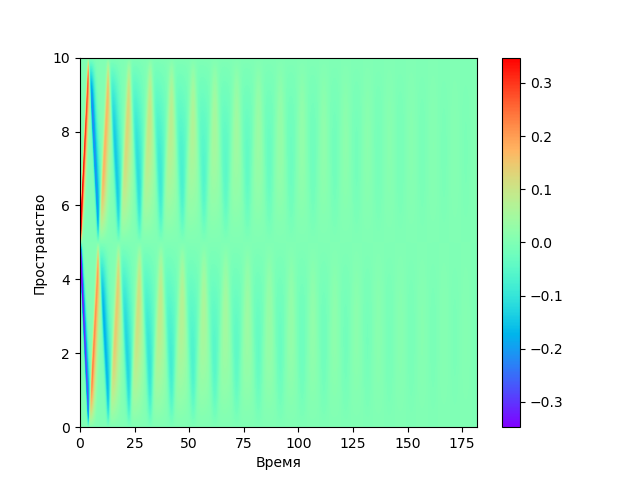
\includegraphics[height=0.4\textheight]{pics/task2/u-2-2-11_1.png}
    \caption{Проекция скорости для $\tau = 0.01, h = 0.01, \mu = 0.1, p(\rho) = \rho$}
\end{figure}

\begin{figure}[H]
    \centering
    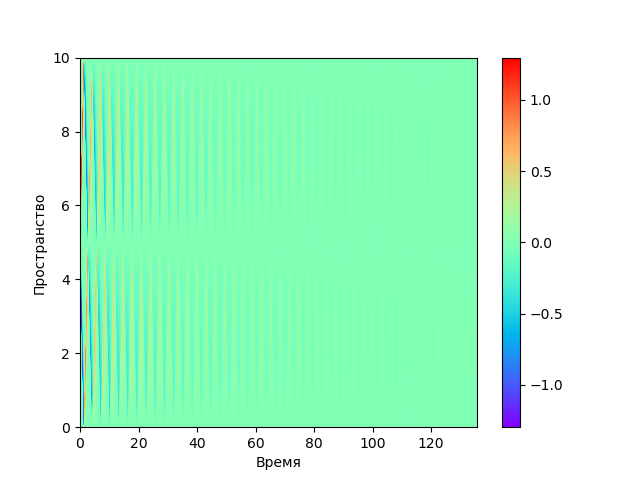
\includegraphics[height=0.4\textheight]{pics/task2/u-2-2-12_1.png}
    \caption{Проекция скорости для $\tau = 0.01, h = 0.01, \mu = 0.1, p(\rho) = 10\rho$}
\end{figure}

\begin{figure}[H]
    \centering
    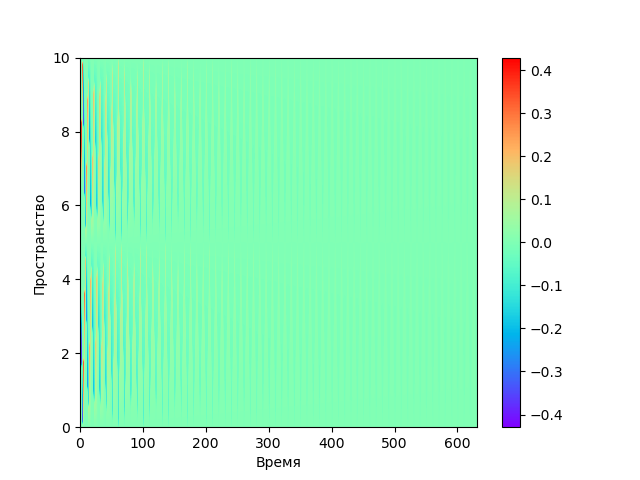
\includegraphics[height=0.4\textheight]{pics/task2/u-2-2-21_1.png}
    \caption{Проекция скорости для $\tau = 0.01, h = 0.01, \mu = 0.01, p(\rho) = \rho$}
\end{figure}

\begin{figure}[H]
    \centering
    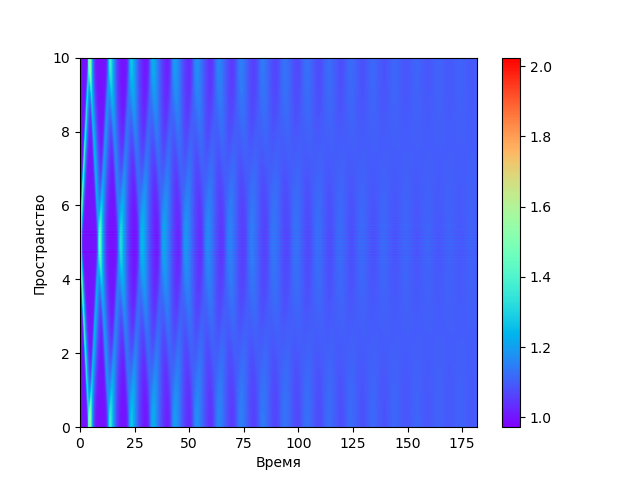
\includegraphics[height=0.4\textheight]{pics/task2/h-2-2-11_1.png}
    \caption{Проекция плотности для $\tau = 0.01, h = 0.01, \mu = 0.1, p(\rho) = \rho$}
\end{figure}

\begin{figure}[H]
    \centering
    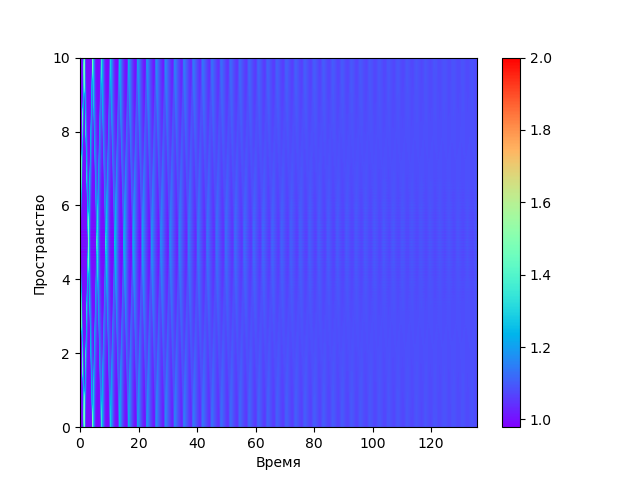
\includegraphics[height=0.4\textheight]{pics/task2/h-2-2-12_1.png}
    \caption{Проекция плотности для $\tau = 0.01, h = 0.01, \mu = 0.1, p(\rho) = 10\rho$}
\end{figure}

\begin{figure}[H]
    \centering
    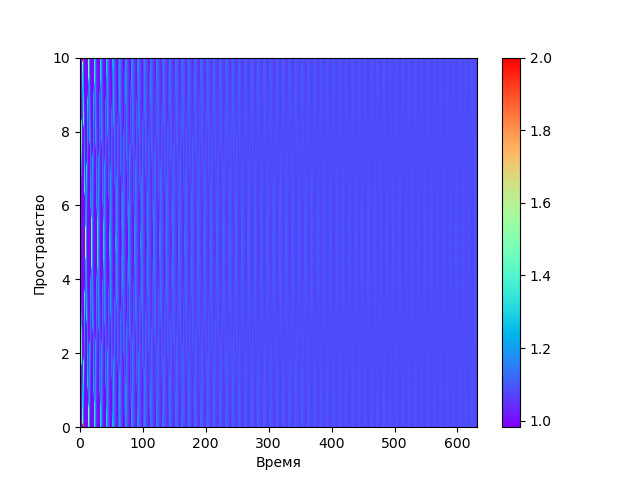
\includegraphics[height=0.4\textheight]{pics/task2/h-2-2-21_1.png}
    \caption{Проекция плотности для $\tau = 0.01, h = 0.01, \mu = 0.01, p(\rho) = \rho$}
\end{figure}
\end{center}

На графиках с одинаковой зависимостью $p$ от $\rho$ видно, что длина цикла примерно одинакова и лежит между 9 и 10, но при этом при меньшей вязкости стабилизация происходит медленнее. При большем коэффициенте зависимости длина цикла уменьшилась.

\begin{figure}[h]
	\begin{minipage}[h]{0.47\linewidth}
		\centering
		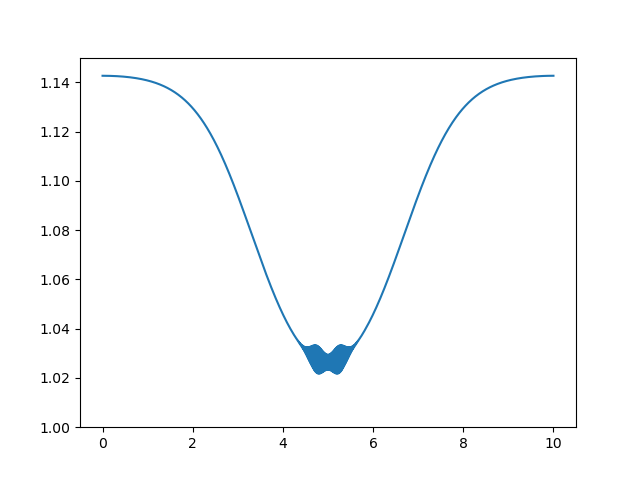
\includegraphics[width=1\linewidth]{pics/task2/14h_1.png} 
		\caption{Плотность на слое $n_{st} / 4$}
	\end{minipage}
	\hfill
	\begin{minipage}[h]{0.47\linewidth}
		\centering
		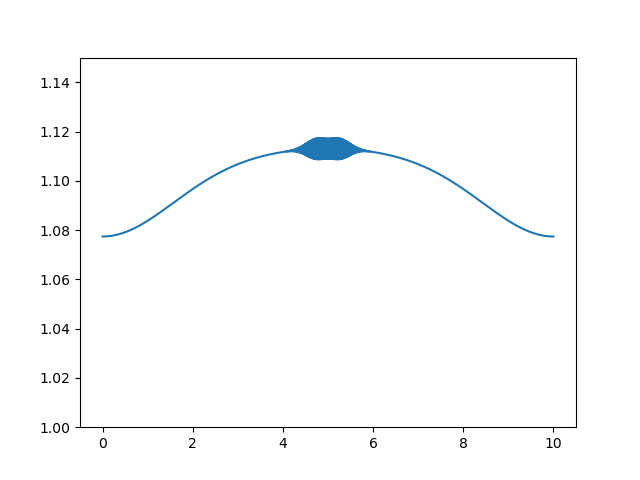
\includegraphics[width=1\linewidth]{pics/task2/24h_1.png} 
		\caption{Плотность на слое $n_{st} / 2$}
	\end{minipage}
	\vfill
	\begin{minipage}[h]{0.47\linewidth}
		\centering
		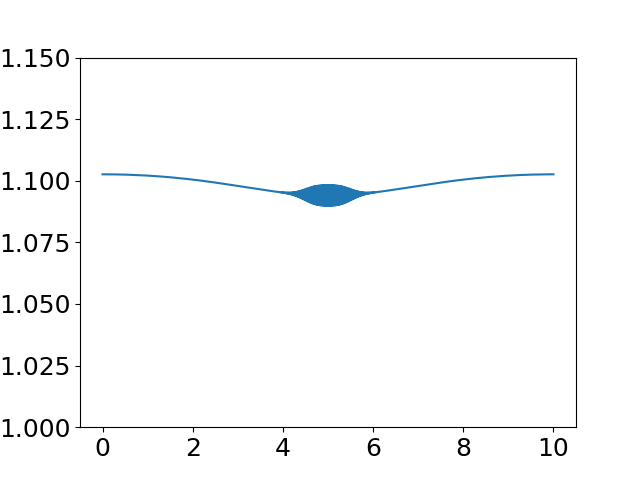
\includegraphics[width=1\linewidth]{pics/task2/34h_1.png} 
		\caption{Плотность на слое $3n_{st} / 4$}
	\end{minipage}
	\hfill
	\begin{minipage}[h]{0.47\linewidth}
		\centering
		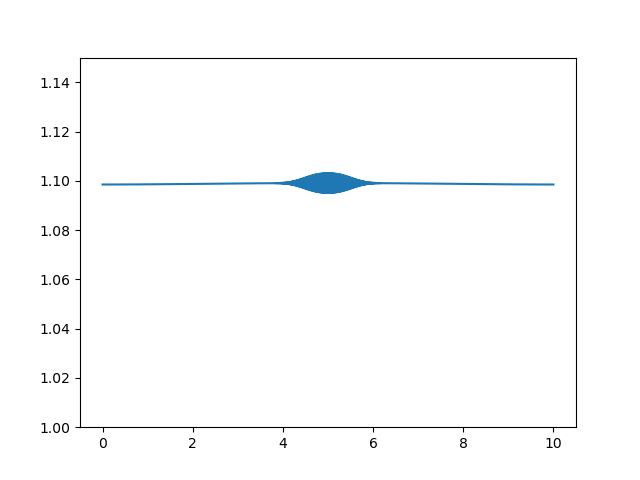
\includegraphics[width=1\linewidth]{pics/task2/44h_1.png} 
		\caption{Плотность на слое $n_{st}$}
	\end{minipage}
	\caption{Графики плотности для $\tau = 0.01, h = 0.01, \mu = 0.1, p(\rho) = \rho$}
\end{figure}

\begin{figure}[h]
	\begin{minipage}[h]{0.47\linewidth}
		\centering
		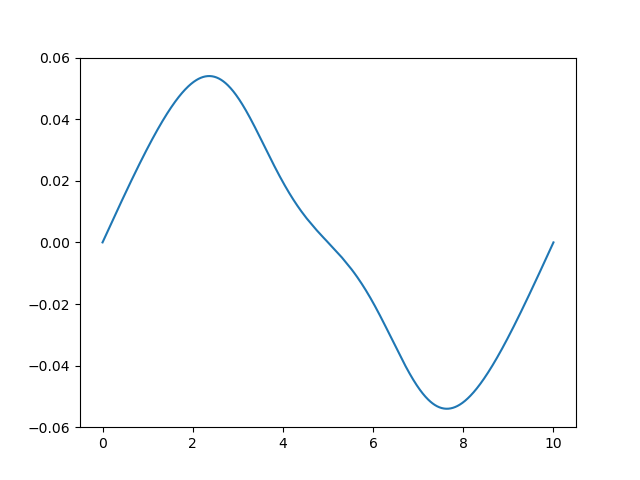
\includegraphics[width=1\linewidth]{pics/task2/14u_1.png} 
		\caption{Скорость на слое $n_{st} / 4$}
	\end{minipage}
	\hfill
	\begin{minipage}[h]{0.47\linewidth}
		\centering
		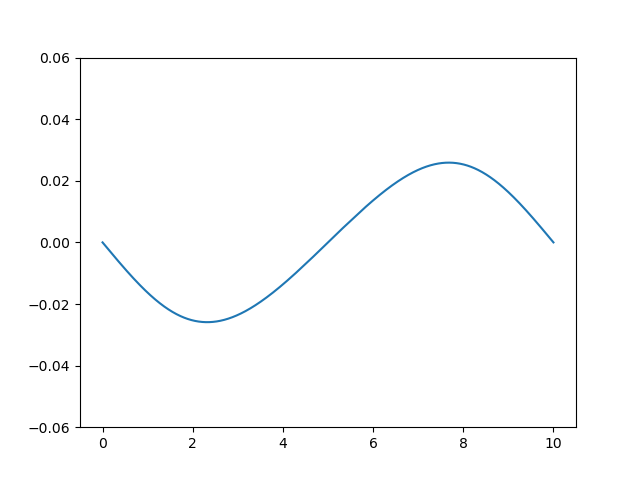
\includegraphics[width=1\linewidth]{pics/task2/24u_1.png} 
		\caption{Скорость на слое $n_{st} / 2$}
	\end{minipage}
	\vfill
	\begin{minipage}[h]{0.47\linewidth}
		\centering
		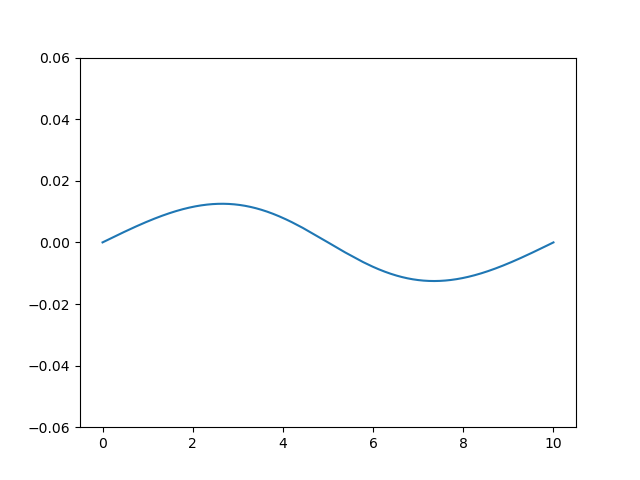
\includegraphics[width=1\linewidth]{pics/task2/34u_1.png} 
		\caption{Скорость на слое $3n_{st} / 4$}
	\end{minipage}
	\hfill
	\begin{minipage}[h]{0.47\linewidth}
		\centering
		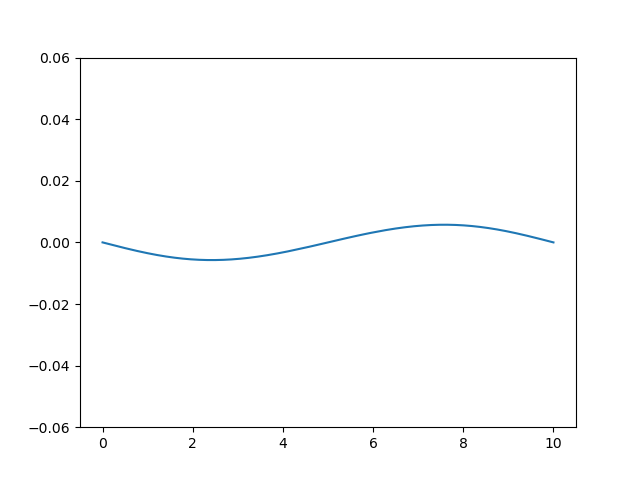
\includegraphics[width=1\linewidth]{pics/task2/44u_1.png} 
		\caption{Скорость на слое $n_{st}$}
	\end{minipage}
	\caption{Графики скорости для $\tau = 0.01, h = 0.01, \mu = 0.1, p(\rho) = \rho$}
\end{figure}

\subsection{Вторая задача}
\subsubsection{$\mu = 0.1, p(\rho) = \rho $}
\begin{tabular}{*{6}{|l}|}
    \hline
    \multicolumn{6}{|c|}{$h = 0.1, \tau = 0.1$} \\
    \hline
    &$n_{st}/4 $&$ n_{st}/2$&$3n_{st}/4$&$n_{st}$&$T_{st}$ \\
    \hline
    $\|\cdot \|$& $1.057994e-01$ & $4.497699e-02$ & $2.105080e-02$ & $9.937196e-03$ &$475.300000$\\
\hline
$\triangle_{mass}$& $-2.151764e-02$ & $-2.169077e-02$ & $-2.170753e-02$ & $-2.171401e-02$ &\\
\hline
\end{tabular}

$\|v-v^{4}\|_{C_h} = 6.210459e-02$


\begin{tabular}{*{6}{|l}|}
    \hline
    \multicolumn{6}{|c|}{$h = 0.01, \tau = 0.01$} \\
    \hline
    &$n_{st}/4 $&$ n_{st}/2$&$3n_{st}/4$&$n_{st}$&$T_{st}$ \\
    \hline
    $\|\cdot \|$& $8.115221e-02$ & $3.328051e-02$ & $1.690131e-02$ & $9.974448e-03$ &$439.410000$\\
\hline
$\triangle_{mass}$& $-2.523587e-03$ & $-2.565776e-03$ & $-2.574194e-03$ & $-2.576565e-03$ &\\
\hline
\end{tabular}

$\|v-v^{4}\|_{C_h} = 7.383419e-03$

\begin{tabular}{*{6}{|l}|}
    \hline
    \multicolumn{6}{|c|}{$h = 0.01, \tau = 0.001$} \\
    \hline
    &$n_{st}/4 $&$ n_{st}/2$&$3n_{st}/4$&$n_{st}$&$T_{st}$ \\
    \hline
    $\|\cdot \|$& $8.448036e-02$ & $3.432835e-02$ & $1.725112e-02$ & $9.996768e-03$ &$439.318000$\\
\hline
$\triangle_{mass}$& $-2.568542e-04$ & $-2.650773e-04$ & $-2.666425e-04$ & $-2.669819e-04$ &\\
\hline
\end{tabular}

$\|v-v^{3}\|_{C_h} = 1.323868e-03$

\subsubsection{$\mu = 0.1, p(\rho) = 10\rho $}

\begin{tabular}{*{6}{|l}|}
    \hline
    \multicolumn{6}{|c|}{$ = 0.1, \tau = 0.01$} \\
    \hline
    &$n_{st}/4 $&$ n_{st}/2$&$3n_{st}/4$&$n_{st}$&$T_{st}$ \\
    \hline
$\|\cdot \|$& $1.298147e-01$ & $5.389401e-02$ & $2.525908e-02$ & $9.947040e-03$ &$289.360000$\\
\hline
$\triangle_{mass}$& $-2.602626e-03$ & $-2.598529e-03$ & $-2.582382e-03$ & $-2.574958e-03$ &\\
\hline
\end{tabular}

$\|v-v^{4}\|_{C_h} = 2.998523e-02$

\begin{tabular}{*{6}{|l}|}
    \hline
    \multicolumn{6}{|c|}{$h = 0.01, \tau = 0.01$} \\
    \hline
    &$n_{st}/4 $&$ n_{st}/2$&$3n_{st}/4$&$n_{st}$&$T_{st}$ \\
    \hline
    $\|\cdot \|$& $8.459588e-02$ & $5.396960e-02$ & $3.536468e-02$ & $9.987376e-03$ &$286.210000$\\
\hline
$\triangle_{mass}$& $-2.345968e-03$ & $-2.415463e-03$ & $-2.440618e-03$ & $-2.445535e-03$ &\\
\hline
\end{tabular}

$\|v-v^{4}\|_{C_h} = 5.722661e-03$

\begin{tabular}{*{6}{|l}|}
    \hline
    \multicolumn{6}{|c|}{$h = 0.01, \tau = 0.001$} \\
    \hline
    &$n_{st}/4 $&$ n_{st}/2$&$3n_{st}/4$&$n_{st}$&$T_{st}$ \\
    \hline
    $\|\cdot \|$& $8.780402e-02$ & $5.311081e-02$ & $3.559624e-02$ & $9.992142e-03$ &$286.119000$\\
\hline
$\triangle_{mass}$& $-2.475217e-04$ & $-2.437268e-04$ & $-2.524342e-04$ & $-2.513063e-04$ &\\
\hline
\end{tabular}
$\|v-v^{3}\|_{C_h} = 2.622959e-03$

\subsubsection{$\mu = 0.1, p(\rho) = 100\rho $}

\begin{tabular}{*{6}{|l}|}
    \hline
    \multicolumn{6}{|c|}{$h = 0.01, \tau = 0.001$} \\
    \hline
    &$n_{st}/4 $&$ n_{st}/2$&$3n_{st}/4$&$n_{st}$&$T_{st}$ \\
    \hline
    $\|\cdot \|$& $8.653968e-02$ & $5.630521e-02$ & $4.426884e-02$ & $9.966610e-03$ &$217.502000$\\
\hline
$\triangle_{mass}$& $-2.296218e-04$ & $-2.474407e-04$ & $-2.469809e-04$ & $-2.491424e-04$ &\\
\hline
\end{tabular}

$\|v-v^{4}\|_{C_h} = 4.344025e-03$

\begin{tabular}{*{6}{|l}|}
    \hline
    \multicolumn{6}{|c|}{$h = 0.001, \tau = 0.001$} \\
    \hline
    &$n_{st}/4 $&$ n_{st}/2$&$3n_{st}/4$&$n_{st}$&$T_{st}$ \\
    \hline
    $\|\cdot \|$& $1.351982e-01$ & $5.697122e-02$ & $2.724762e-02$ & $9.986078e-03$ &$216.503000$\\
\hline
$\triangle_{mass}$& $-2.303206e-04$ & $-2.431240e-04$ & $-2.462610e-04$ & $-2.474967e-04$ &\\
\hline
\end{tabular}

$\|v-v^{2}\|_{C_h} = 2.747033e-03$

\subsubsection{$\mu = 0.1, p(\rho) = \rho^{1.4} $}
\begin{tabular}{*{6}{|l}|}
    \hline
    \multicolumn{6}{|c|}{$h = 0.1, \tau = 0.1$} \\
    \hline
    &$n_{st}/4 $&$ n_{st}/2$&$3n_{st}/4$&$n_{st}$&$T_{st}$ \\
    \hline
    $\|\cdot \|$& $8.849004e-02$ & $4.460481e-02$ & $2.274127e-02$ & $9.816406e-03$ &$386.600000$\\
\hline
$\triangle_{mass}$& $-2.142117e-02$ & $-2.194042e-02$ & $-2.194306e-02$ & $-2.197424e-02$ &\\
\hline
\end{tabular}

$\|v-v^{4}\|_{C_h} = 1.089634e-01$

\begin{tabular}{*{6}{|l}|}
    \hline
    \multicolumn{6}{|c|}{$h = 0.01, \tau = 0.01$} \\
    \hline
    &$n_{st}/4 $&$ n_{st}/2$&$3n_{st}/4$&$n_{st}$&$T_{st}$ \\
    \hline
    $\|\cdot \|$& $8.177089e-02$ & $4.732491e-02$ & $2.412279e-02$ & $9.999100e-03$ &$384.230000$\\
\hline
$\triangle_{mass}$& $-2.475776e-03$ & $-2.528510e-03$ & $-2.528038e-03$ & $-2.532089e-03$ &\\
\hline
\end{tabular}

$\|v-v^{4}\|_{C_h} = 1.319770e-02$

\begin{tabular}{*{6}{|l}|}
    \hline
    \multicolumn{6}{|c|}{$h = 0.01, \tau = 0.001$} \\
    \hline
    &$n_{st}/4 $&$ n_{st}/2$&$3n_{st}/4$&$n_{st}$&$T_{st}$ \\
    \hline
    $\|\cdot \|$& $8.999629e-02$ & $4.564517e-02$ & $2.333583e-02$ & $9.999805e-03$ &$392.287000$\\
\hline
$\triangle_{mass}$& $-2.703800e-04$ & $-2.551330e-04$ & $-2.638645e-04$ & $-2.623066e-04$ &\\
\hline
\end{tabular}

$\|v-v^{3}\|_{C_h} = 1.200642e-03$

\begin{tabular}{*{6}{|l}|}
    \hline
    \multicolumn{6}{|c|}{$h = 0.001, \tau = 0.01$} \\
    \hline
    &$n_{st}/4 $&$ n_{st}/2$&$3n_{st}/4$&$n_{st}$&$T_{st}$ \\
    \hline
$\|\cdot \|$& $8.171681e-02$ & $4.723875e-02$ & $2.407144e-02$ & $9.998224e-03$ &$384.230000$\\
\hline
$\triangle_{mass}$& $-2.463330e-03$ & $-2.500851e-03$ & $-2.507733e-03$ & $-2.510269e-03$ &\\
\hline  
\end{tabular}

$\|v-v^{3}\|_{C_h} = 1.281673e-02$

\subsubsection{$\mu = 0.01, p(\rho) = \rho $}

\begin{tabular}{*{6}{|l}|}
    \hline
    \multicolumn{6}{|c|}{$h = 0.01, \tau = 0.01$} \\
    \hline
    &$n_{st}/4 $&$ n_{st}/2$&$3n_{st}/4$&$n_{st}$&$T_{st}$ \\
    \hline
$\|\cdot \|$& $3.755305e-02$ & $2.563334e-02$ & $2.026205e-02$ & $9.988237e-03$ &$1147.100000$\\
\hline
$\triangle_{mass}$& $-2.257917e-02$ & $-2.262130e-02$ & $-2.264216e-02$ & $-2.264381e-02$ &\\
\hline
\end{tabular}

$\|v-v^{4}\|_{C_h} = 1.498957e-01$

\begin{tabular}{*{6}{|l}|}
    \hline
    \multicolumn{6}{|c|}{$h = 0.01, \tau = 0.001$} \\
    \hline
    &$n_{st}/4 $&$ n_{st}/2$&$3n_{st}/4$&$n_{st}$&$T_{st}$ \\
    \hline
    $\|\cdot \|$& $4.756873e-02$ & $2.231827e-02$ & $1.895506e-02$ & $9.999852e-03$ &$1187.069000$\\
\hline
$\triangle_{mass}$& $-2.737012e-03$ & $-2.731282e-03$ & $-2.728745e-03$ & $-2.733232e-03$ &\\
\hline
\end{tabular}

$\|v-v^{3}\|_{C_h} = 3.385155e-02$

\begin{tabular}{*{6}{|l}|}
    \hline
    \multicolumn{6}{|c|}{$h = , \tau = $} \\
    \hline
    &$n_{st}/4 $&$ n_{st}/2$&$3n_{st}/4$&$n_{st}$&$T_{st}$ \\
    \hline
    $\|\cdot \|$& $4.624345e-02$ & $2.465977e-02$ & $1.436130e-02$ & $9.993862e-03$ &$1242.180000$\\
\hline
$\triangle_{mass}$& $-2.249926e-02$ & $-2.254468e-02$ & $-2.255458e-02$ & $-2.255879e-02$ &\\
\hline
\end{tabular}

$\|v-v^{2}\|_{C_h} = 1.291567e-01$

\subsubsection{$\mu = 0.01, p(\rho) = 10\rho $}

\begin{tabular}{*{6}{|l}|}
    \hline
    \multicolumn{6}{|c|}{$h = 0.1, \tau = 0.001$} \\
    \hline
    &$n_{st}/4 $&$ n_{st}/2$&$3n_{st}/4$&$n_{st}$&$T_{st}$ \\
    \hline
$\|\cdot \|$& $6.888265e-02$ & $3.459087e-02$ & $1.825954e-02$ & $9.997479e-03$ &$693.024000$\\
\hline
$\triangle_{mass}$& $-2.631510e-03$ & $-2.570296e-03$ & $-2.565111e-03$ & $-2.545413e-03$ &\\
\hline

\end{tabular}

$\|v-v^{4}\|_{C_h} = 1.399669e-01$

\begin{tabular}{*{6}{|l}|}
    \hline
    \multicolumn{6}{|c|}{$h = , \tau = $} \\
    \hline
    &$n_{st}/4 $&$ n_{st}/2$&$3n_{st}/4$&$n_{st}$&$T_{st}$ \\
    \hline
    $\|\cdot \|$& $4.596806e-02$ & $2.721373e-02$ & $2.582281e-02$ & $9.997545e-03$ &$577.493000$\\
\hline
$\triangle_{mass}$& $-2.456556e-03$ & $-2.470025e-03$ & $-2.479802e-03$ & $-2.479199e-03$ &\\
\hline
\end{tabular}

 $\|v-v^{3}\|_{C_h} = 1.267514e-01$
\subsubsection{$\mu = 0.01, p(\rho) = 100\rho $}

\begin{tabular}{*{6}{|l}|}
    \hline
    \multicolumn{6}{|c|}{$h = 0.01, \tau = 0.0001$} \\
    \hline
    &$n_{st}/4 $&$ n_{st}/2$&$3n_{st}/4$&$n_{st}$&$T_{st}$ \\
    \hline
$\|\cdot \|$& $7.214288e-02$ & $2.692124e-02$ & $1.536680e-02$ & $9.998859e-03$ &$480.526600$\\
\hline
$\triangle_{mass}$& $-2.426798e-04$ & $-2.481020e-04$ & $-2.495873e-04$ & $-2.502651e-04$ &\\
\hline
\end{tabular}

$\|v-v^{2}\|_{C_h} = 5.224555e-02$

\subsubsection{$\mu = 0.01, p(\rho) = \rho^{1.4} $}

\begin{tabular}{*{6}{|l}|}
    \hline
    \multicolumn{6}{|c|}{$h = 0.1, \tau = 0.01$} \\
    \hline
    &$n_{st}/4 $&$ n_{st}/2$&$3n_{st}/4$&$n_{st}$&$T_{st}$ \\
    \hline$\|\cdot \|$& $6.206453e-02$ & $2.635210e-02$ & $1.491993e-02$ & $9.996229e-03$ &$948.120000$\\
\hline
$\triangle_{mass}$& $-2.140423e-02$ & $-2.139353e-02$ & $-2.137896e-02$ & $-2.136954e-02$ &\\
\hline
\end{tabular}
$\|v-v^{4}\|_{C_h} = 1.350754e-01$

\begin{tabular}{*{6}{|l}|}
    \hline
    \multicolumn{6}{|c|}{$h = 0.01, \tau = 0.001$} \\
    \hline
    &$n_{st}/4 $&$ n_{st}/2$&$3n_{st}/4$&$n_{st}$&$T_{st}$ \\
    \hline$\|\cdot \|$& $3.638901e-02$ & $2.530445e-02$ & $2.101946e-02$ & $9.997771e-03$ &$990.525000$\\
\hline
$\triangle_{mass}$& $-2.634875e-03$ & $-2.648825e-03$ & $-2.642002e-03$ & $-2.645937e-03$ &\\
\hline
\end{tabular}

$\|v-v^{2}\|_{C_h} = 4.821490e-02$

\subsubsection{$\mu = 0.001, p(\rho) = \rho $}

\begin{tabular}{*{6}{|l}|}
    \hline
    \multicolumn{6}{|c|}{$h = 0.01, \tau = 0.001$} \\
    \hline
    &$n_{st}/4 $&$ n_{st}/2$&$3n_{st}/4$&$n_{st}$&$T_{st}$ \\
    \hline$\|\cdot \|$& $3.293496e-02$ & $1.889809e-02$ & $1.569922e-02$ & $9.999973e-03$ &$1849.610000$\\
\hline
$\triangle_{mass}$& $-2.126218e-02$ & $-2.128896e-02$ & $-2.129372e-02$ & $-2.129839e-02$ &\\
\hline
\end{tabular}

$\|v-v^{3}\|_{C_h} = 9.548446e-02$

\begin{tabular}{*{6}{|l}|}
    \hline
    \multicolumn{6}{|c|}{$h = 0.001, \tau = 0.0001$} \\
    \hline
    &$n_{st}/4 $&$ n_{st}/2$&$3n_{st}/4$&$n_{st}$&$T_{st}$ \\
    \hline
$\|\cdot \|$& $7.943369e-02$ & $3.416127e-02$ & $2.313465e-02$ & $1.861502e-02$ &$1000.000000$\\
\hline
$\triangle_{mass}$& $-3.133873e-03$ & $-3.152216e-03$ & $-3.156661e-03$ & $-3.158007e-03$ &\\
\hline   
   \end{tabular}

$\|v-v^{1}\|_{C_h} = 1.189583e-01$

\subsubsection{$\mu = 0.001, p(\rho) = 10\rho $}

\begin{tabular}{*{6}{|l}|}
    \hline
    \multicolumn{6}{|c|}{$h = 0.01, \tau = 0.0001$} \\
    \hline
    &$n_{st}/4 $&$ n_{st}/2$&$3n_{st}/4$&$n_{st}$&$T_{st}$ \\
    \hline
$\|\cdot \|$& $5.654326e-02$ & $2.418228e-02$ & $1.529745e-02$ & $9.999739e-03$ &$748.537500$\\
\hline
$\triangle_{mass}$& $-2.407347e-03$ & $-2.424248e-03$ & $-2.428702e-03$ & $-2.430007e-03$ &\\
\hline
\end{tabular}

$\|v-v^{2}\|_{C_h} = 1.636180e-01$

\subsubsection{$\mu = 0.001, p(\rho) = 100\rho $}

Я не подобрал сетку, на которой вычисления происходили бы достаточно быстро и не расходились.

\subsubsection{$\mu = 0.001, p(\rho) = \rho^{1.4} $}
\begin{tabular}{*{6}{|l}|}
    \hline
    \multicolumn{6}{|c|}{$h = 0.01, \tau = 0.0001$} \\
    \hline
    &$n_{st}/4 $&$ n_{st}/2$&$3n_{st}/4$&$n_{st}$&$T_{st}$ \\
    \hline
    $\|\cdot \|$& $6.623326e-01$ & $3.439675e-01$ & $2.141368e-01$ & $1.480272e-01$ &$100.000000$\\
\hline
$\triangle_{mass}$& $-2.337562e-03$ & $-2.729491e-03$ & $-2.792877e-03$ & $-2.810747e-03$ &\\
\hline
\end{tabular}

$\|v-v^{2}\|_{C_h} = 3.783958e-01$

\subsubsection{Графики}
\begin{center}
\begin{figure}[H]
    \centering
    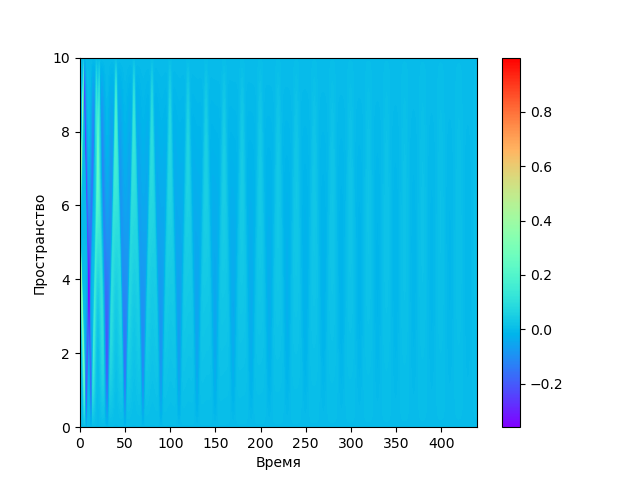
\includegraphics[height=0.4\textheight]{pics/task2/u-2-2-11_2.png}
    \caption{Проекция скорости для $\tau = 0.01, h = 0.01, \mu = 0.1, p(\rho) = \rho$}
\end{figure}

\begin{figure}[H]
    \centering
    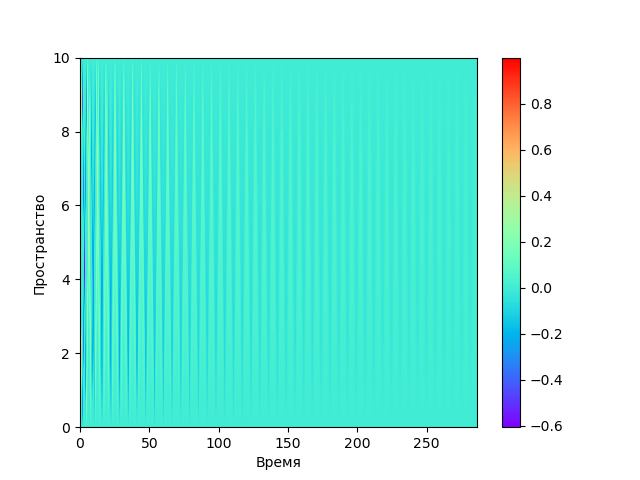
\includegraphics[height=0.4\textheight]{pics/task2/u-2-2-12_2.png}
    \caption{Проекция скорости для $\tau = 0.01, h = 0.01, \mu = 0.1, p(\rho) = 10\rho$}
\end{figure}

\begin{figure}[H]
    \centering
    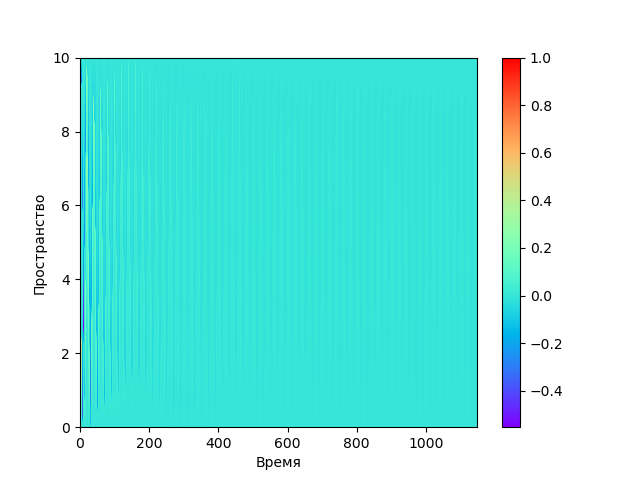
\includegraphics[height=0.4\textheight]{pics/task2/u-2-2-21_2.png}
    \caption{Проекция скорости для $\tau = 0.01, h = 0.01, \mu = 0.01, p(\rho) = \rho$}
\end{figure}

\begin{figure}[H]
    \centering
    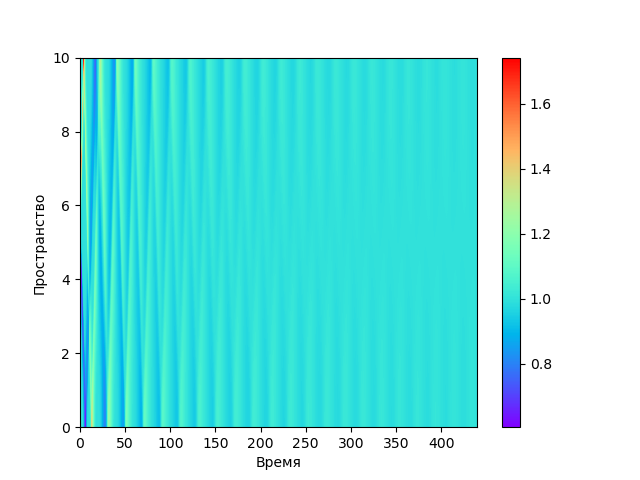
\includegraphics[height=0.4\textheight]{pics/task2/h-2-2-11_2.png}
    \caption{Проекция плотности для $\tau = 0.01, h = 0.01, \mu = 0.1, p(\rho) = \rho$}
\end{figure}

\begin{figure}[H]
    \centering
    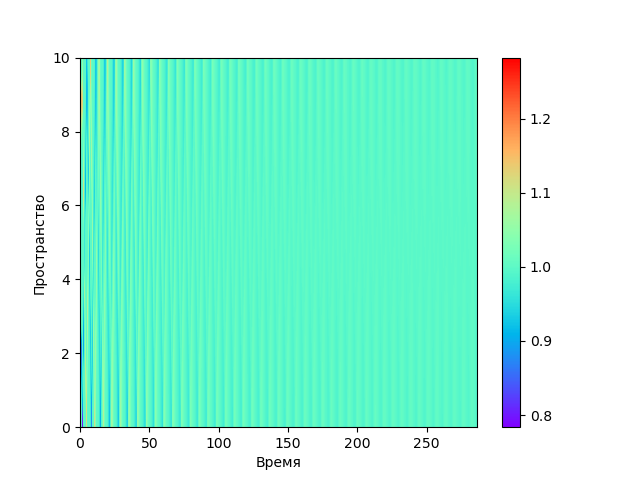
\includegraphics[height=0.4\textheight]{pics/task2/h-2-2-12_2.png}
    \caption{Проекция плотности для $\tau = 0.01, h = 0.01, \mu = 0.1, p(\rho) = 10\rho$}
\end{figure}

\begin{figure}[H]
    \centering
    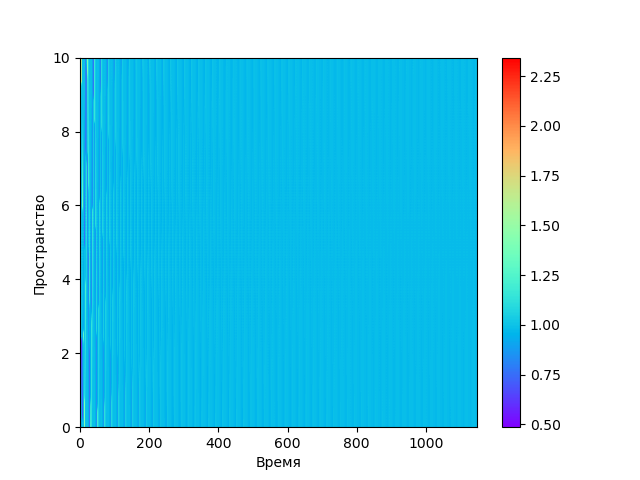
\includegraphics[height=0.4\textheight]{pics/task2/h-2-2-21_2.png}
    \caption{Проекция плотности для $\tau = 0.01, h = 0.01, \mu = 0.01, p(\rho) = \rho$}
\end{figure}
\end{center}


\begin{figure}[h]
	\begin{minipage}[h]{0.47\linewidth}
		\centering
		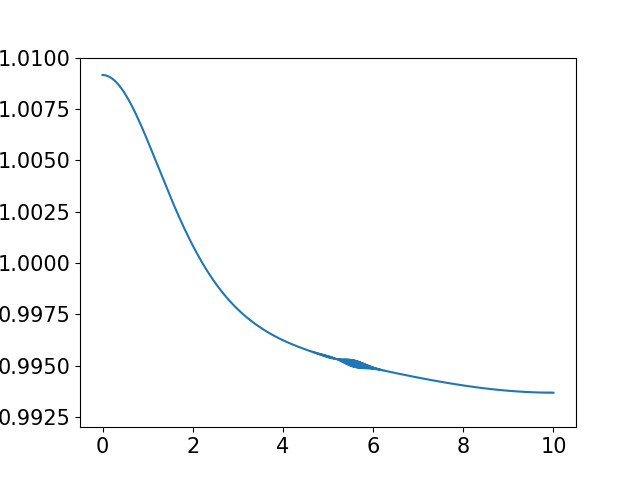
\includegraphics[width=1\linewidth]{pics/task2/14h_2.png} 
		\caption{Плотность на слое $n_{st} / 4$}
	\end{minipage}
	\hfill
	\begin{minipage}[h]{0.47\linewidth}
		\centering
		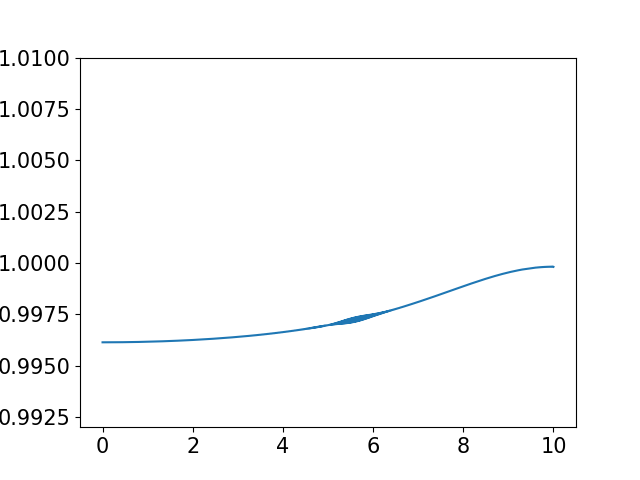
\includegraphics[width=1\linewidth]{pics/task2/24h_2.png} 
		\caption{Плотность на слое $n_{st} / 2$}
	\end{minipage}
	\vfill
	\begin{minipage}[h]{0.47\linewidth}
		\centering
		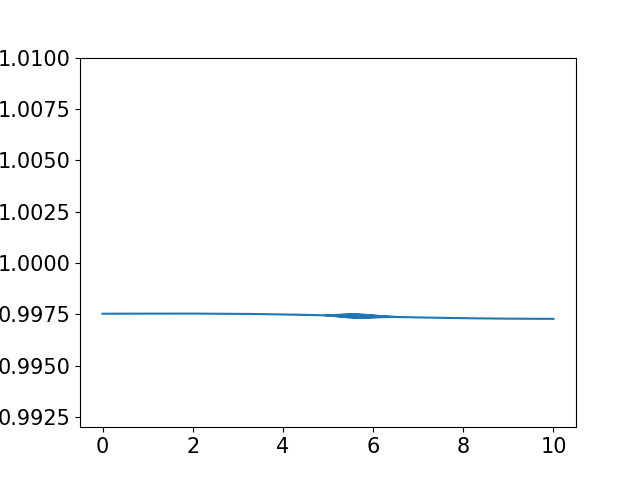
\includegraphics[width=1\linewidth]{pics/task2/34h_2.png} 
		\caption{Плотность на слое $3n_{st} / 4$}
	\end{minipage}
	\hfill
	\begin{minipage}[h]{0.47\linewidth}
		\centering
		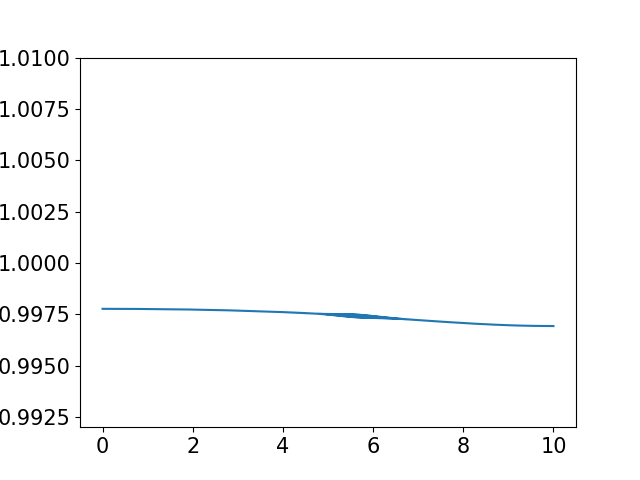
\includegraphics[width=1\linewidth]{pics/task2/44h_2.png} 
		\caption{Плотность на слое $n_{st}$}
	\end{minipage}
	\caption{Графики плотности для $\tau = 0.01, h = 0.01, \mu = 0.1, p(\rho) = \rho$}
\end{figure}

\begin{figure}[h]
	\begin{minipage}[h]{0.47\linewidth}
		\centering
		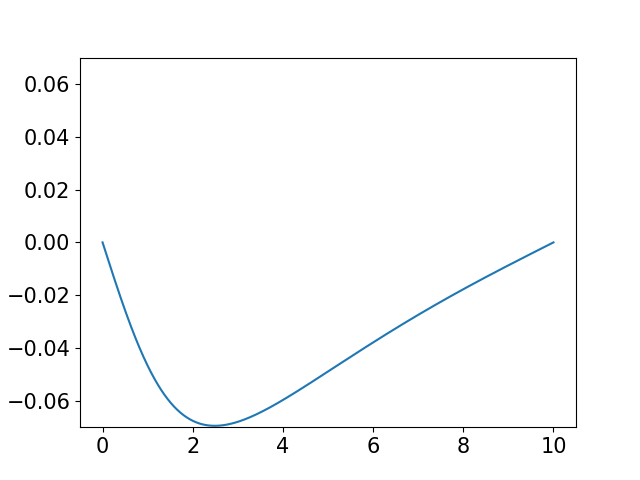
\includegraphics[width=1\linewidth]{pics/task2/14u_2.png} 
		\caption{Скорость на слое $n_{st} / 4$}
	\end{minipage}
	\hfill
	\begin{minipage}[h]{0.47\linewidth}
		\centering
		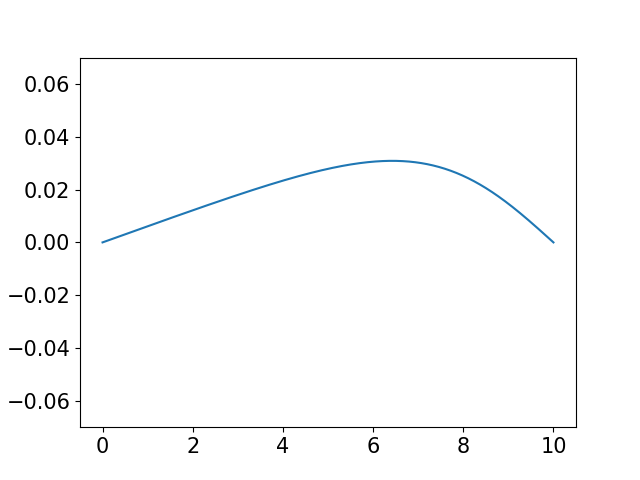
\includegraphics[width=1\linewidth]{pics/task2/24u_2.png} 
		\caption{Скорость на слое $n_{st} / 2$}
	\end{minipage}
	\vfill
	\begin{minipage}[h]{0.47\linewidth}
		\centering
		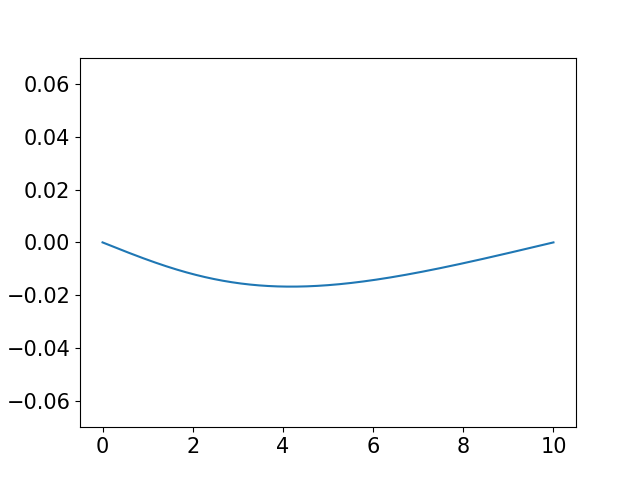
\includegraphics[width=1\linewidth]{pics/task2/34u_2.png} 
		\caption{Скорость на слое $3n_{st} / 4$}
	\end{minipage}
	\hfill
	\begin{minipage}[h]{0.47\linewidth}
		\centering
		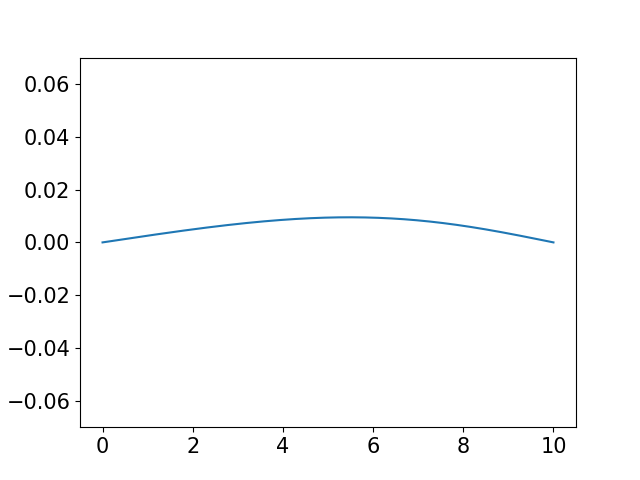
\includegraphics[width=1\linewidth]{pics/task2/44u_2.png} 
		\caption{Скорость на слое $n_{st}$}
	\end{minipage}
	\caption{Графики скорости для $\tau = 0.01, h = 0.01, \mu = 0.1, p(\rho) = \rho$}
\end{figure}


